\begin{figure}
    \centering
    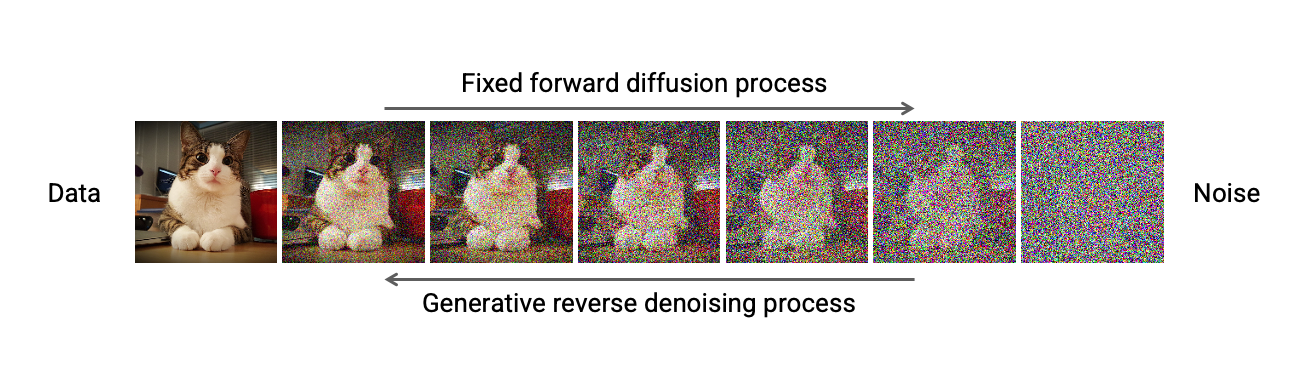
\includegraphics[width=\textwidth]{00_images/diffusion.png}
    \caption{Denoising Diffusion Process}
    \label{fig:denoising_diffusion_process}
\end{figure}

\section{Introduction}
The advent of generative artificial intelligence (AI) has been transformative across various domains, ranging from education \cite{baidoo-anu_education_2023, qadir_engineering_2023, lim_generative_2023} to workplaces \cite{noy_experimental_2023, brynjolfsson_generative_2023} and daily activities \cite{dwivedi_opinion_2023}. Central to this transformation is deep learning, a key pillar enabling AI to analyze and synthesize complex data patterns. Initially, generative AI is defined by its ability to create new, original data samples that reflect the statistical characteristics of a specified dataset, represented mathematically as: given a sample $x$ from distribution $q(x)$, the generative model produces outputs $\hat{x}$ that appear to be drawn from $q(x)$ \cite{luo_understanding_2022}.

Following this introductory note on generative AI, the focus shifts to time-series forecasting, an area of critical importance across various industries. Time-series data, characterized by their temporal dependencies and multifaceted interactions, present unique challenges and opportunities for forecasting future events based on historical data. This is particularly significant in fields such as healthcare prediction \cite{penfold_use_2013, bui_time_2018, che_recurrent_2018, kaushik_ai_2020, chimmula_time_2020, zeroual_deep_2020}, energy management \cite{deb_review_2017, chou_forecasting_2018, wang_diffload_2023}, and traffic control \cite{lippi_short-term_2013, pavlyuk_short-term_2017}.

In the landscape of time-series forecasting, the solution space has evolved considerably over time. Initial advancements were marked by the introduction of Long Short-Term Memory (LSTM) variants, notably, the Seq2Seq Autoencoder-LSTM \cite{sutskever_sequence_2014}. However, a significant paradigm shift occurred in 2017 with the introduction of the Transformer structure, which incorporated attention mechanisms \cite{vaswani_attention_2017}. This innovation addressed the critical limitation of LSTMs, which was the loss of previous information over extended sequences \cite{murray_state---art_2023}. Subsequent developments in Transformer-based models, \cite{nguyen_temporal_2021, zhou_informer_2021, wu_autoformer_2022, zhou_fedformer_2022, zhang_crossformer_2022, nie_time_2023}, have furthered the field. 

In the field of generative modeling, the introduction of modeling structures such as variational autoencoders (VAEs), normalizing flows (NFs), and generative adversarial networks (GANs) have marked significant advancements \cite{foster_generative_2022, bond-taylor_deep_2022}. Yet, the emergence of diffusion models signals a revolutionary period, promising superior-quality outputs that are pushing the state-of-the-art \cite{dhariwal_diffusion_2021, yang_diffusion_2023, croitoru_diffusion_2023}. A diffusion model can be characterized by the fact that they simulate, as the name implies, a diffusion process transforming data into white noise and then reversing it back into data as shown in \autoref{fig:denoising_diffusion_process}.
These models, capable of approximating the original data distribution, have shown exceeding results in various domains, including image \cite{ho_cascaded_2021, dhariwal_diffusion_2021, rombach_high-resolution_2022, austin_structured_2021}, text \cite{gong_diffuseq_2023, li_diffusion-lm_2022, yu_latent_2023}, speech \cite{kong_diffwave_2020, yang_diffsound_2023} and video synthesis \cite{yang_diffusion_2022, harvey_flexible_2022, ho_imagen_2022, ho_video_2022}.

In this paper, we narrow our focus to the application of diffusion models in time-series forecasting. These models, distinguished by their profound ability to comprehend intricate data dynamics, are revolutionizing this field \cite{lin_diffusion_2023, koo_comprehensive_2023}. First time-series forecasting is further formalized together with how to evaluate the models in sub-section \ref{sec:time-series}. Afterwards, the intrinsic workings of the diffusion model and how to condition it is explained in section \ref{sec:preliminary}. Then the diffusion-based time-series forecasting papers are discussed in section \ref{sec:diffusion_time-series}. Finally, a comprehensive discussion and future works is given in sections \ref{sec:discussion} and \ref{sec:future_works} respectively.

The main contributions of this paper are:
\begin{itemize}
    \item In-depth preliminary section about diffusion models and the methods of conditioning that are used for time-series modeling.
    \item A chronologically ordered overview of the diffusion models capable of time-series forecasting, going in-depth on the implementation in relation to the preliminary, specify the results on which datasets, and a discussion about the work in relation to other diffusion models. 
    \item The work serves as in depth overview for researchers seeking to acquaint themselves with the methods that make up the current state-of-the-art diffusion models for time-series forecasting. 
\end{itemize}

\subsection{Time-series} \label{sec:time-series}
Time-series modeling, as highlighted by \textcite{koo_comprehensive_2023, lin_diffusion_2023}, is a specialized form of conditional generative modeling, where segments of the time-series are used to generate other segments. This area encompasses three key types: generation, imputation, and forecasting. Generation is about creating synthetic time-series data; imputation deals with filling gaps in existing data, and forecasting is the prediction of future values. These types are interconnected, with forecasting being a specific form of imputation and both imputation and forecasting being aspects of generation. This section will delve into the problem definition for time-series forecasting and evaluation metrics to assess model performance.

\begin{figure}[hb]
\centering
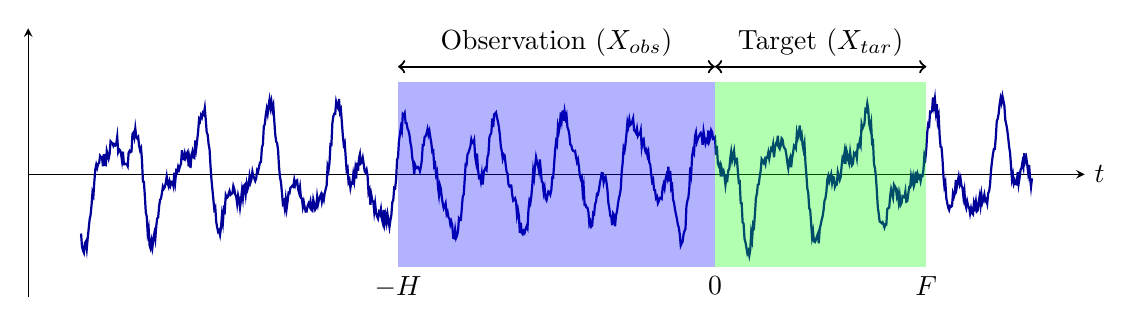
\begin{tikzpicture}
    \begin{axis}[
        axis lines=middle,
        ticks=none,
        width=15cm, height=5cm,
        xmin=0, xmax=100,
        ymin=-1.6, ymax=1.9,
        xlabel=$t$,
        every axis x label/.style={at={(ticklabel* cs:1)},anchor=west},
        every axis y label/.style={at={(ticklabel* cs:1)},anchor=south},
    ]

    \addplot[thick, blue!60!black, domain=5:95, samples=1000] {
        0.5*sin(deg(0.9*x)) 
        + 0.3*sin(deg(2*x)) 
        + 0.2*cos(deg(3*x)) 
        % + 0.2*sin(deg(5*x)) 
        + 0.1*rand
    };

    \fill[blue, opacity=0.3] (axis cs:35,-1.2) rectangle (axis cs:65,1.2);
    \fill[green, opacity=0.3] (axis cs:65,-1.2) rectangle (axis cs:85,1.2); 

    % Moved the annotations within the axis limits
    \draw[<->, thick] (axis cs:35,1.4) -- (axis cs:65,1.4) node[midway, above] {Observation ($X_{obs}$)};
    \draw[<->, thick] (axis cs:65,1.4) -- (axis cs:85,1.4) node[midway, above] {Target ($X_{tar}$)};

    % Add extra labels below the squares
    \node[below] at (axis cs:35,-1.2) {$-H$};
    \node[below] at (axis cs:65,-1.2) {$0$};
    \node[below] at (axis cs:85,-1.2) {$F$};
    \end{axis}
\end{tikzpicture}
\caption{Example of univariate time-series forecasting situation.}
\label{fig:time-series-univariate}
\end{figure}

\subsubsection{Problem definition for Time-series Forecasting} \label{sec:time-series_problem_definition}
Since time is inherently continuous, these series are represented through discrete time steps, determined by a chosen sampling frequency, which can range from milliseconds to hours. For simplicity we assume that the entire dataset $X$ is discretized evenly in the rest of the paper if not explicitly specified. The historical time range, comprising $H$ steps, is defined as the set of observations $obs = \left\{t \in \mathbb{Z} \mid -H < t \leq 0\right\}$, while the future range, spanning $F$ steps, is denoted as the targets $tar = \left\{t \in \mathbb{Z} \mid 0 < t \leq F\right\}$. Consequently, historical data can be represented as $X_{obs} \in \mathbb{R}^{d \times H}$, and the target forecast data as $X_{tar} \in \mathbb{R}^{d \times F}$, where $d$ indicates the number of distinct features. A time-series is classified as univariate when $d = 1$ as illustrated in \autoref{fig:time-series-univariate}, and as multivariate when $d > 1$. In this context, a specific value at time step $t$ and feature $i$ from the time-series can be defined as $x_{i,t}$, where $i \in \left\{1 \dots d\right\}$ and $t \in \left\{-H, \ldots, F\right\}$ or as $x_t$ when talking about the entire value vector at the time step.


\subsubsection{Evaluation Metrics} \label{sec:time-series_evaluation_metric}
The evaluation of time-series forecasting can be done through a varaiaty of metrics. The most common ones are through the use of the Mean Squared Error (MSE), Mean Absolute Error (MAE), and the Continuous Ranked Probability Score (CRPS) \cite{winkler_scoring_1996}. The biggest difference between these metrics is that the MSE \& MAE focus on the mean error, while the CRPS also takes into account the uncertainty of the prediction. 

The MSE and MAE over a time-series forecasting are defined as:
% \begin{align}
%     \text{MSE}(\hat{X}_{tar}, X_{tar}) &= \frac{1}{F} \sum\limits_{t=0}^{F} (x_t - \hat{x}_t)^2 \\
%     \text{MAE}(\hat{X}_{tar}, X_{tar}) &= \frac{1}{F}\sum_{t=0}^{F} \left| x_t - \hat{x}_t \right|
% \end{align}
\begin{equation} \label{eq:mse}
    \text{MSE}(\hat{X}_{tar}, X_{tar}) = \frac{1}{F} \sum\limits_{t=0}^{F} (x_t - \hat{x}_t)^2
    \qquad \qquad
    \text{MAE}(\hat{X}_{tar}, X_{tar}) = \frac{1}{F}\sum_{t=0}^{F} \left| x_t - \hat{x}_t \right|
\end{equation}


The output of these error measurements are vectors for the multivariate time-series, at end the average over all features is taken as the final value. One must consider that the values ought to be normalized, as otherwise errors of different features can have very different scales.

The CRPS is a metric that is used for probabilistic forecasting and measures the compatibility of a cumulative distribution function (CDF) $F$ with an observation $X_{tar}$. In other words, the CRPS metric becomes smaller if the distribution is highly concentrated on the prediction as illustrated in \autoref{fig:crps_vizualization}. However, in many scenarios the CDF $F$ is not available analytically, but only by estimating it through a set of $N$ forecast samples $\hat{X}_{tar}^N$ \cite{jordan_evaluating_2019}. These samples are gathered by sampling the probabilistic model $N$ times.
The CRPS metric is calculated for of a single feature at a single timestamp. It is possible to estimate the empirical CDF $\hat{F}_N(z)$ given a point $z$ from these predictions. The empirical CDF at a point $z$ is estimated by the proportion of forecast values that are less than or equal to $z$ and is defined as
\begin{equation}
\hat{F}_{i,t}^N(z) = \frac{1}{N} \sum_{n=1}^{N} \mathbb{I}\{\hat{x}_{i,t}^n \leq z\}.
\end{equation}
Where $\mathbb{I}\{\hat{X}_{i,t}^i \leq z\}$ is the indicator function that equals 1 if the condition $\hat{X}_{tar}^i \leq z$ is true, and 0 otherwise.
The CRPS for the empirical CDF $\hat{F}_N$ and the observation $X_{tar}$ is then calculated as:
\begin{equation} \label{eq:crps}
\text{CRPS}(\hat{F}_{i,t}^N, x_{i,t}) = \int_{\mathbb{R}} \left( \hat{F}_{i,t}^N(z) - \mathbb{I}\{x_{i,t} \leq z\} \right)^2 dz
\end{equation}
Where $i$ indicates the feature and $t$ the timestamp of the forecasts. The estimation of this formulation is further explained and optimized by \textcite{jordan_evaluating_2019}.

As previously mentioned, the CRPS focuses on a single feature at a specific timestamp. To transform this for a multivariate time-series forecast with multiple timestamps in the future some normalization and averaging ought to be done. This can be either done as the Normalized Average CRPS, which is formulated as such:
\begin{equation} \label{eq:nacrps}
    \text{NACRPS}(\hat{F}^N, X_{tar}) = \frac{\sum_{i,t} \text{CRPS}(\hat{F}_{i,t}^N, x_{i,t})}{\sum_{i,t} |x_{i,t}|}
\end{equation}
And then there is the CRPS-sum, which is the CRPS for the distribution F for the sum of all $d$ features:
\begin{equation} \label{eq:crps-sum}
    \text{CRPS}_\text{sum}(\hat{F}^N, X_{tar}) = \frac{\sum_{t} \text{CRPS}(\hat{F}_{i,t}^N, \sum_{i} x_i)}{\sum_{i,t} |x_{i,t}|}
\end{equation}


\begin{figure}[!t]
    \centering
    \begin{minipage}{0.5\textwidth}
        \centering
        \begin{tikzpicture}
            \begin{axis}[
                width=0.7\linewidth, % Set the width of the graph
                height=0.65\linewidth, % Set the height of the graph
                axis lines=middle, % Middle aligned axis
                axis line style={draw=none}, % No border around the graph
                xlabel=, % x-axis label
                ylabel=, % y-axis label
                xtick={1,3,5}, % x-axis ticks for z-1, z, z+1
                xticklabels={$z-1$,$z$,$z+1$}, % x-axis tick labels
                ytick={0,0.25,0.5,0.75,1}, % y-axis ticks
                ymin=0, ymax=1, % y-axis limits
                xmin=0, xmax=7, % x-axis limits
                clip=false, % Prevents clipping of paths
                grid=both, % Add grid lines
                grid style={gray!30}, % Gray grid lines
            ]
        
            % Blue line
            \addplot[name path=blue, blue, thick, sharp plot, update limits=false] coordinates {(0,0) (3,0) (3,1) (6,1)};
        
            % Red line (Gaussian CDF)
            \addplot[name path=red, red, smooth, domain=0:6] {normcdf(x,3,1)};
        
            % Fill area between blue and red line
            \addplot[red!10] fill between[of=blue and red];
        
            % Arrow to the blue line
            \draw[<-] (axis cs:2.5,0.1) -- (axis cs:1.2,0.3) node[above] {$\text{CRPS}(\hat{F}_{i,t}^N, x_{i,t})$};
        
            % Arrow to the red line
            \draw[<-] (axis cs:4,0.8) -- (axis cs:5,0.7) node[right] {$\hat{F}_{i,t}^N$};
        
            % Arrow to the fill between
            \draw[<-] (axis cs:3.2,0.3) -- (axis cs:4.2,0.2) node[right] {$\mathbb{I}\{x_{i,t} \leq z\}$};
        
            \end{axis}
        \end{tikzpicture}
    \end{minipage}\hfill
    \begin{minipage}{0.5\textwidth}
        \centering
        \begin{tikzpicture}
            \begin{axis}[
                width=0.7\linewidth, % Set the width of the graph
                height=0.65\linewidth, % Set the height of the graph
                axis lines=middle, % Middle aligned axis
                axis line style={draw=none}, % No border around the graph
                xlabel=, % x-axis label
                ylabel=, % y-axis label
                xtick={1,3,5}, % x-axis ticks for z-1, z, z+1
                xticklabels={$z-1$,$z$,$z+1$}, % x-axis tick labels
                ytick={0,0.25,0.5,0.75,1}, % y-axis ticks
                ymin=0, ymax=1, % y-axis limits
                xmin=0, xmax=7, % x-axis limits
                clip=false, % Prevents clipping of paths
                grid=both, % Add grid lines
                grid style={gray!30}, % Gray grid lines
            ]
        
            % Blue line
            \addplot[name path=blue, blue, thick, sharp plot, update limits=false] coordinates {(0,0) (3,0) (3,1) (6,1)};
        
            % Red line (Gaussian CDF)
            \addplot[name path=red, red, smooth, domain=0:6] {normcdf(x,3,0.5)};
        
            % Fill area between blue and red line
            \addplot[red!10] fill between[of=blue and red];
        
            \end{axis}
        \end{tikzpicture}
    \end{minipage}
    \caption{Comparative Visualization of Continuous Ranked Probability Scores: The left plot exhibits a higher CRPS value, indicated by the greater area between the forecast distribution (red line) and the step function (blue line), compared to the right plot.} \label{fig:crps_vizualization}
\end{figure}
